% Standalone vector figure; compile with XeLaTeX from this directory.
% Component icons are original schematic drawings, not official AWS icons.
% Architecture sources: docs/architecture.md and infra/*.yaml.
\documentclass[tikz,border=8pt]{standalone}
\usepackage{fontspec}
\setmainfont{texgyreheros-regular.otf}[BoldFont=texgyreheros-bold.otf]
\usetikzlibrary{arrows.meta,backgrounds,fit}
\definecolor{ink}{HTML}{26384A}
\definecolor{accent}{HTML}{32658A}
\definecolor{border}{HTML}{CAD5DF}
\definecolor{cloudblue}{HTML}{F3F7FB}
\definecolor{iconfill}{HTML}{E7EFF6}
\newcommand{\componenticon}[1]{%
  \tikz[draw=accent,fill=accent,line width=0.8pt,baseline=-2pt]{%
    \fill[iconfill,rounded corners=3pt] (-.48,-.43) rectangle (.48,.43);
    \pic {#1};}}
\definecolor{blue}{HTML}{2463B2}
\definecolor{green}{HTML}{168469}
\definecolor{orange}{HTML}{DD751F}
\definecolor{purple}{HTML}{7550B6}
\definecolor{olive}{HTML}{628D2C}
\newcommand{\serviceicon}[2]{\begingroup\colorlet{accent}{#1}\colorlet{iconfill}{#1!12}\scalebox{1.55}{\componenticon{#2}}\endgroup}
\begin{document}
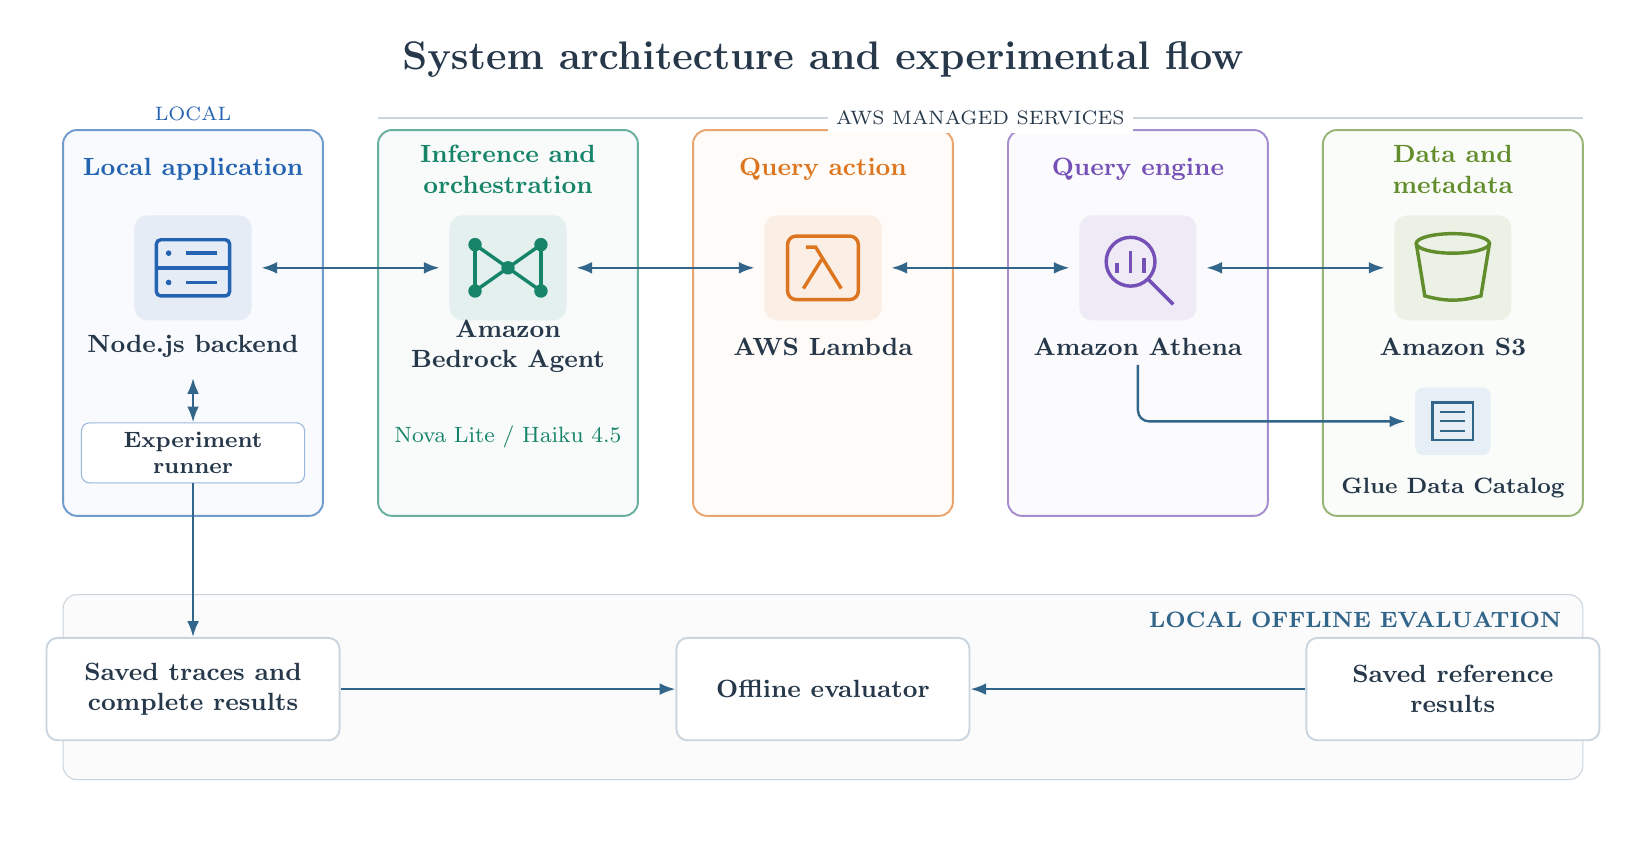
\begin{tikzpicture}[
  font=\small,text=ink,
  box/.style={draw=border,line width=.7pt,fill=white,rounded corners=4pt,align=center,
    text width=2.5cm,minimum height=1.85cm,inner sep=6pt,font=\small\bfseries},
  flow/.style={-{Latex[length=2mm]},draw=accent,line width=.85pt,rounded corners=4pt},
  both/.style={{Latex[length=2mm]}-{Latex[length=2mm]},draw=accent,line width=.85pt,rounded corners=4pt},
  pics/browser/.style={code={
    \draw[rounded corners=1pt] (-.34,-.23) rectangle (.34,.23);
    \draw (-.34,.10)--(.34,.10);
    \fill (-.25,.16) circle (.018); \fill (-.17,.16) circle (.018);
    \draw (-.12,-.02)--(-.19,-.08)--(-.12,-.14);
    \draw (.12,-.02)--(.19,-.08)--(.12,-.14);
  }},
  pics/server/.style={code={
    \draw[rounded corners=1pt] (-.30,-.23) rectangle (.30,.23);
    \draw (-.30,0)--(.30,0);
    \fill (-.20,.12) circle (.023); \fill (-.20,-.12) circle (.023);
    \draw (-.06,.12)--(.20,.12); \draw (-.06,-.12)--(.20,-.12);
  }},
  pics/database/.style={code={
    \draw (0,.17) ellipse [x radius=.29,y radius=.09];
    \draw (-.29,.17)--(-.29,-.18) arc[start angle=180,end angle=360,x radius=.29,y radius=.09]--(.29,.17);
    \draw (-.29,0) arc[start angle=180,end angle=360,x radius=.29,y radius=.09];
  }},
  pics/agent/.style={code={
    \draw (-.27,.19)--(0,0)--(.27,.19);
    \draw (-.27,-.19)--(0,0)--(.27,-.19);
    \draw (-.27,.19)--(-.27,-.19) (.27,.19)--(.27,-.19);
    \foreach \x/\y in {-.27/.19,-.27/-.19,.27/.19,.27/-.19,0/0}
      \fill (\x,\y) circle (.055);
  }},
  pics/function/.style={code={
    \draw (-.14,.17)--(-.06,.17)--(.15,-.17);
    \draw (-.01,.07)--(-.16,-.17);
    \draw[rounded corners=2pt] (-.29,-.26) rectangle (.29,.26);
  }},
  pics/search/.style={code={
    \draw (-.06,.05) circle (.20);
    \draw (.08,-.09)--(.29,-.30);
    \draw (-.17,-.04)--(-.17,.04) (-.06,-.04)--(-.06,.14) (.05,-.04)--(.05,.08);
  }},
  pics/catalog/.style={code={
    \draw (-.26,-.24) rectangle (.26,.24);
    \draw (-.16,.12)--(.16,.12) (-.16,0)--(.16,0) (-.16,-.12)--(.16,-.12);
  }},
  pics/bucket/.style={code={
    \draw (0,.20) ellipse [x radius=.30,y radius=.08];
    \draw (-.30,.20)--(-.23,-.23) to[bend right=15] (.23,-.23)--(.30,.20);
  }}
]


\begin{scope}[on background layer]
  \fill[white] (-2.1,3.2) rectangle (18.1,-6.8);
\end{scope}
\node[font=\Large\bfseries] at (8,2.8) {System architecture and experimental flow};
\foreach \x/\col/\title in {0/blue/Local application,4/green/Inference and orchestration,8/orange/Query action,12/purple/Query engine,16/olive/Data and metadata} {
  \path[draw=\col!65,fill=\col!3,rounded corners=5pt,line width=.7pt]
    (\x-1.65,1.9) rectangle (\x+1.65,-3.0);
  \node[text=\col,font=\small\bfseries,align=center,text width=3cm] at (\x,1.4) {\title};
}
\node[font=\scriptsize,text=blue] at (0,2.1) {LOCAL};
\draw[draw=border,line width=.6pt] (2.35,2.05)--(17.65,2.05);
\node[fill=white,font=\scriptsize,text=ink,inner sep=3pt] at (10,2.05) {AWS MANAGED SERVICES};
\node (backend) at (0,.15) {\serviceicon{blue}{server}};
\node (agent) at (4,.15) {\serviceicon{green}{agent}};
\node (lambda) at (8,.15) {\serviceicon{orange}{function}};
\node (athena) at (12,.15) {\serviceicon{purple}{search}};
\node (s3) at (16,.15) {\serviceicon{olive}{bucket}};
\foreach \x/\txt in {0/Node.js backend,4/Amazon Bedrock Agent,8/AWS Lambda,12/Amazon Athena,16/Amazon S3}
  \node[font=\small\bfseries,align=center,text width=3.1cm] (label\x) at (\x,-.85) {\txt};
\node[draw=blue!45,fill=white,rounded corners=3pt,align=center,text width=2.6cm,minimum height=.6cm,font=\footnotesize\bfseries] (runner) at (0,-2.2) {Experiment runner};
\node[font=\footnotesize,align=center,text=green] at (4,-2.0) {Nova Lite / Haiku 4.5};
\node (glue) at (16,-1.8) {\componenticon{catalog}};
\node[font=\footnotesize\bfseries] at (16,-2.65) {Glue Data Catalog};
\draw[both] (backend)--(agent);
\draw[both] (agent)--(lambda);
\draw[both] (lambda)--(athena);
\draw[both] (athena)--(s3);
\draw[both] (runner.north)--(0,-1.25);
\draw[flow] (label12.south)--(12,-1.8)--(glue.west);
\path[draw=border,fill=gray!3,rounded corners=5pt] (-1.65,-4.0) rectangle (17.65,-6.35);
\node[anchor=north east,font=\footnotesize\bfseries,text=accent] at (17.5,-4.1) {LOCAL OFFLINE EVALUATION};
\node[box,text width=3.3cm,minimum height=1.3cm] (saved) at (0,-5.2) {Saved traces and\\complete results};
\node[box,text width=3.3cm,minimum height=1.3cm] (eval) at (8,-5.2) {Offline evaluator};
\node[box,text width=3.3cm,minimum height=1.3cm] (gold) at (16,-5.2) {Saved reference\\results};
\draw[flow] (runner)--(saved);
\draw[flow] (saved)--(eval);
\draw[flow] (gold)--(eval);
\end{tikzpicture}
\end{document}
